% Created 2023-10-01 Sun 17:31
% Intended LaTeX compiler: pdflatex
\documentclass[12pt, a4paper]{article}
\usepackage[utf8]{inputenc}
\usepackage[T1]{fontenc}
\usepackage{graphicx}
\usepackage{longtable}
\usepackage{wrapfig}
\usepackage{rotating}
\usepackage[normalem]{ulem}
\usepackage{amsmath}
\usepackage{amssymb}
\usepackage{capt-of}
\usepackage{hyperref}
\usepackage{placeins}
\usepackage{gensymb}
\usepackage[letterpaper]{geometry}
\geometry{top=1.0in, bottom=1.0in, left=1.0in, right=1.0in}
\usepackage{rotating}
\usepackage{graphicx}
\usepackage{pgfplots}
\usepackage{subcaption}
\usepackage{filecontents}
\usepackage{tikz}
\usepackage{fancyhdr}
\usepackage{enumitem}
\pagestyle{fancy}
\lhead{}
\chead{}
\rhead{Johnson \thepage}
\lfoot{}
\cfoot{}
\rfoot{}
\renewcommand{\headrulewidth}{0pt}
\renewcommand{\footrulewidth}{0pt}
\setlength\headsep{0.333in}
\newcommand{\bibent}{\noindent \hangindent 40pt}
\newenvironment{workscited}{\newpage \begin{center} Works Cited \end{center}}{\newpage }
\graphicspath{ {./attachments/} }
\author{Christian}
\date{\today}
\title{}
\hypersetup{
 pdfauthor={Christian},
 pdftitle={},
 pdfkeywords={},
 pdfsubject={},
 pdfcreator={Emacs 28.2.50 (Org mode 9.7-pre)}, 
 pdflang={English}}
\begin{document}

\begin{document}
\begin{flushleft}
Christian Johnson\\
\vspace{2mm}Dr. Paul Crilly\\
\vspace{2mm}Antennas and Propogation\\
\vspace{2mm}September 27 2023\\
\vspace{4mm}\begin{center}
Lab 2 Report
\end{center}
\vspace{1mm}\setlength{\parindent}{0.5in}

\begin{abstract}
This laboratory exercise, focused on measuring transmission line losses, determining the length of transmission lines, and locating faults within them. The experiment was conducted using an Agilent 9912A Field Fox Analyzer and various types of coaxial cables (RG-58, RG-8, RG-213). By comparing physical measurements with electrical measurements, we were able to determine the impact of cable diameter and frequency on losses. Our findings revealed distinct behaviors in RG-58 and RG-213, noting a "critical frequency" at which losses increase significantly. Additionally, fault locations were pinpointed using the N9912A. After examining these results, we were better able to understand the behavior of transmission lines and their suitability for specific applications. This report summarizes our findings, including measurements, observations, and answers to critical questions posed during the lab procedure.
\end{abstract}
\section*{Procedure}
\label{sec:org450acd4}
Transmission lines are foundational components within communication systems, serving as the essential conduits through which signals traverse from their source to their intended destination. This laboratory exercise was designed to deepen our comprehension of these transmission lines and their behaviors. Our exploration involved three distinct cable types, and our aim was to determine various characteristics for each of these lines. These characteristics included electrical length, velocity factor, corrected length, and physical length. Most of our measurements were executed with the use of the N9912A Field Fox Analyzer, while physical measurements were carried out using a measuring tape.

With our initial observations of fundamental characteristics completed, our next task was to examine the cable losses at various frequencies. To achieve this, we used the N9912A Field Fox Analyzer again. This allowed us to conduct precise measurements of signal attenuation over a spectrum of frequencies, ranging from the low-frequency realm of 2 MHz to the much higher frequencies of 20 MHz, 200 MHz, and 2000 MHz. For each cable type—RG-58, RG-8, and RG-213—we measured and recorded the losses at these specified frequencies. The objective was to decipher how these transmission lines respond to different signal frequencies and the corresponding attenuation levels they exhibit. By doing so, we gained valuable insights into the frequency-dependent behavior of each cable, laying the foundation for more informed engineering decisions in real-world scenarios.

Having explored cable losses, we next sought to detect hidden faults within the transmission lines with the N9912A Analyzer. This phase of our experiment provided invaluable insights into the practical aspect of maintaining and troubleshooting communication systems. Identifying the precise location of faults within transmission lines is a critical skill, particularly in scenarios where signal integrity is paramount. We recorded the fault locations obtained through the analyzer and compared them with the actual location, obtaining a result of 3.21 m compared to the actual 3.99 m. This comparative analysis allowed us to assess the accuracy of our fault detection process.
\section*{Results}
\label{sec:org6d15e12}

Throughout this lab experiment, we took several measurements. The first set we took focused on determining the electrical length, velocity factor, corrected length, and physical length of the cables under examination. For the RG-58 cable, we observed an electrical length of 2.7 meters, with a velocity factor of 0.66. The corrected length, accounting for the velocity factor, was calculated to be 1.782 meters, with a physical length of 1.829 meters, resulting in a minor \% error of 2.57\%. Similarly, for the longer RG-58 cable, an electrical length of 23 meters, a velocity factor of 0.66, and a corrected length of 15.18 meters were determined. The physical length closely aligned with the corrected length at 15.54 meters, yielding a \% error of 2.32\%. Notably, the RG-213 cable exhibited an electrical length of 33 meters, a velocity factor of 0.66, and a corrected length of 21.78 meters. The physical length was found to be 21.9 meters, with a remarkably low \% error of 0.54\%. These values can be seen in table 1. 
The next phase of our investigation involved measuring cable losses at varying frequencies (2 MHz, 20 MHz, 200 MHz, and 2 GHz) for both RG-58 and RG-213 cables. In the case of the RG-58 cable, the measured losses exhibited frequency-dependent characteristics. At 2 MHz, the loss was a mere 0.06 dB, corresponding to 0.328 dB/m. However, as the frequency increased, so did the loss, with values reaching 0.15 dB at 20 MHz, 1.3 dB at 200 MHz, and a significant 10.11 dB at 2 GHz. These measurements highlight the frequency sensitivity of the RG-58 cable, with higher frequencies leading to more substantial losses per meter. Similarly, the longer RG-58 cable displayed similar frequency-dependent behavior. At 2 MHz, the loss was 0.2 dB, equating to 0.0129 dB/m. As the frequency escalated, the losses became more pronounced, culminating in 2.3 dB at 20 MHz, 7.7 dB at 200 MHz, and a substantial 17.5 dB at 2 GHz. This data underscores the cable's susceptibility to signal attenuation at higher frequencies. Conversely, the RG-213 cable demonstrated a notably different profile. Its losses were relatively consistent across the tested frequencies. At 2 MHz, the loss measured 0.13 dB, equivalent to 0.0059 dB/m. This trend continued with a loss of 1 dB at 20 MHz, 4.8 dB at 200 MHz, and 14.6 dB at 2 GHz. These findings suggest that the RG-213 cable offers more predictable and stable signal attenuation characteristics, making it suitable for specific applications. These values can be seen in table 2.
We calculated the location of the fault using the same procedure from before, resulting in the formula: (12.1-6.1)(0.535) = 3.21 m. This result is relatively close to the value we measured with a physical measuring tape - at 3.99 m. This demonstrates the method we would use in a practical application to locate a similar fault in a more realistic scenario - such as a powerline onboard a cutter. 
In summary, our measurements helped us to learn about the characteristics of RG-58 and RG-213 coaxial cables, shedding light on their electrical length, velocity factor, corrected length, and cable loss behavior across a range of frequencies. These insights are crucial for engineering decisions, ensuring optimal performance in real-world communication systems.
\section*{Conclusions}
\label{sec:org7fc5436}

In this laboratory exercise, we explored the characteristics and behavior of transmission lines, focusing on RG-58 and RG-213 coaxial cables. Our efforts were directed towards understanding electrical length, velocity factor, corrected length, and cable losses at varying frequencies. Several key insights were gathered from our experiments.

Firstly, concerning the electrical and corrected lengths, it was evident that the velocity factor significantly impacted these parameters. The physical length of the cable was consistently greater than the corrected length due to this factor. This shows the importance of taking such factors into account when performing calculations.

Secondly, the cable loss measurements demonstrateddifferent behaviors for RG-58 and RG-213. RG-58 exhibited a noticeable increase in loss as frequency escalated, underlining its higher susceptibility to signal attenuation at higher frequencies. In contrast, RG-213 displayed more consistent losses across the tested frequencies, suggesting its suitability for applications where stable signal propagation is crucial.

Overall, our experiments underscored the importance of considering cable type, frequency, and length in the design and implementation of communication systems. Understanding the behavior of transmission lines is paramount for achieving optimal system performance, minimizing losses, and ensuring effective signal transmission.

These findings lay a solid foundation for further exploration and application of transmission line theory in practical engineering scenarios, providing valuable insights for optimizing communication systems.


\newpage
\begin{center}
Apendices
\end{center}

\begin{figure}[htb]
\centering
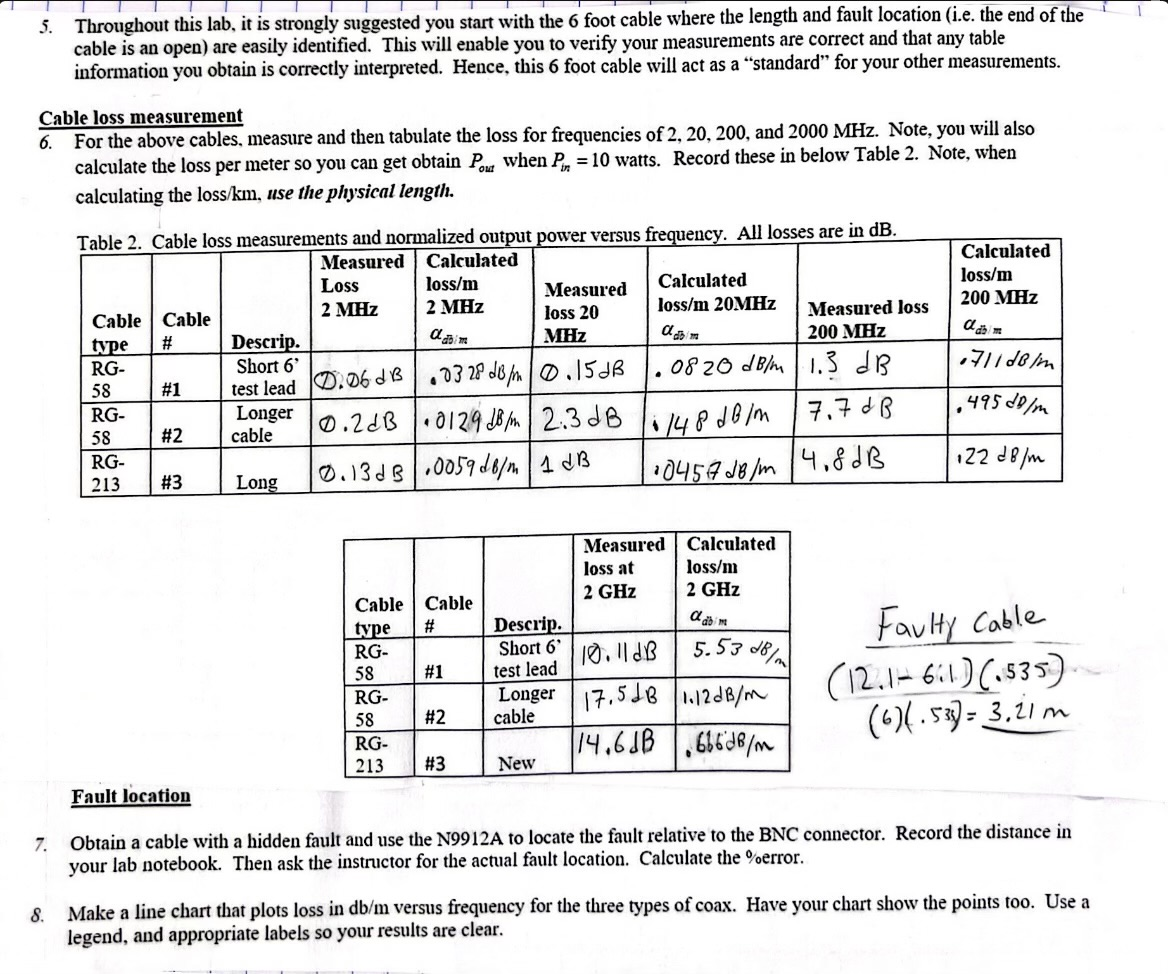
\includegraphics[width=0.7\textwidth]{LabNotebook1.jpg}
\caption{Recorded Data}
\end{figure}

\newpage
\begin{figure}[htb]
\centering
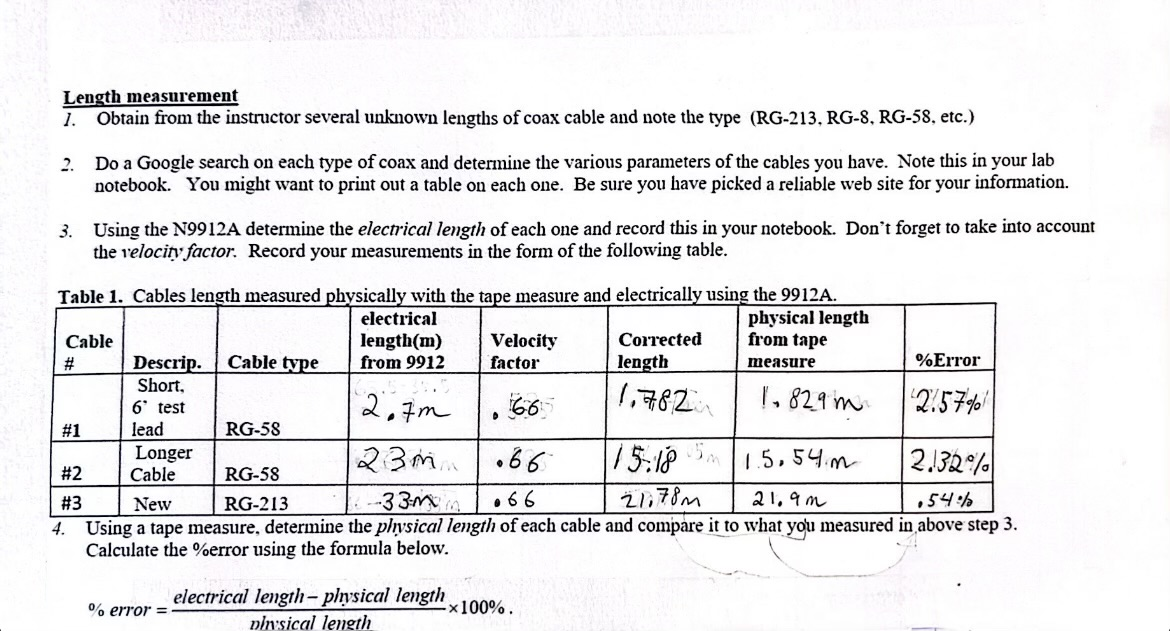
\includegraphics[width=0.6\textwidth]{LabNotebook2.jpg}
\caption{Recorded Data}
\end{figure}
\newpage
\begin{figure}[htb]
\centering
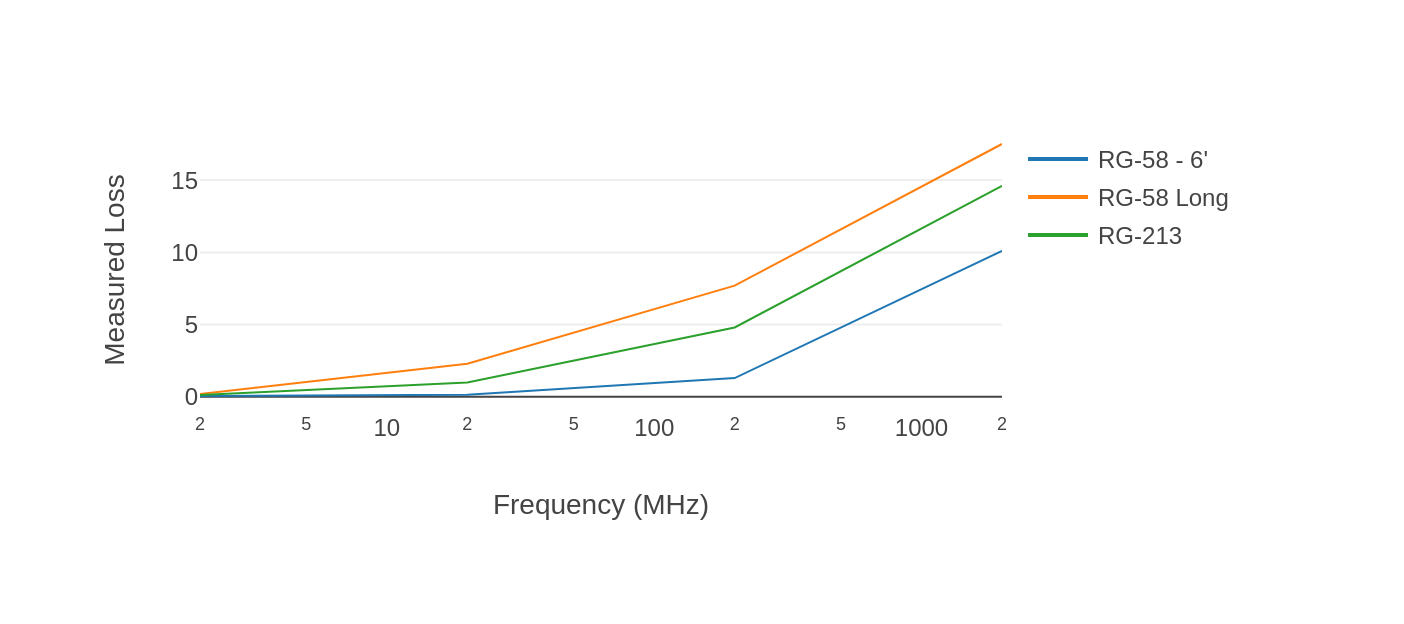
\includegraphics[width=0.6\textwidth]{MeasuredGraph.png}
\caption{Measured Loss and Frequency}
\end{figure}
\begin{figure}[htb]
\centering
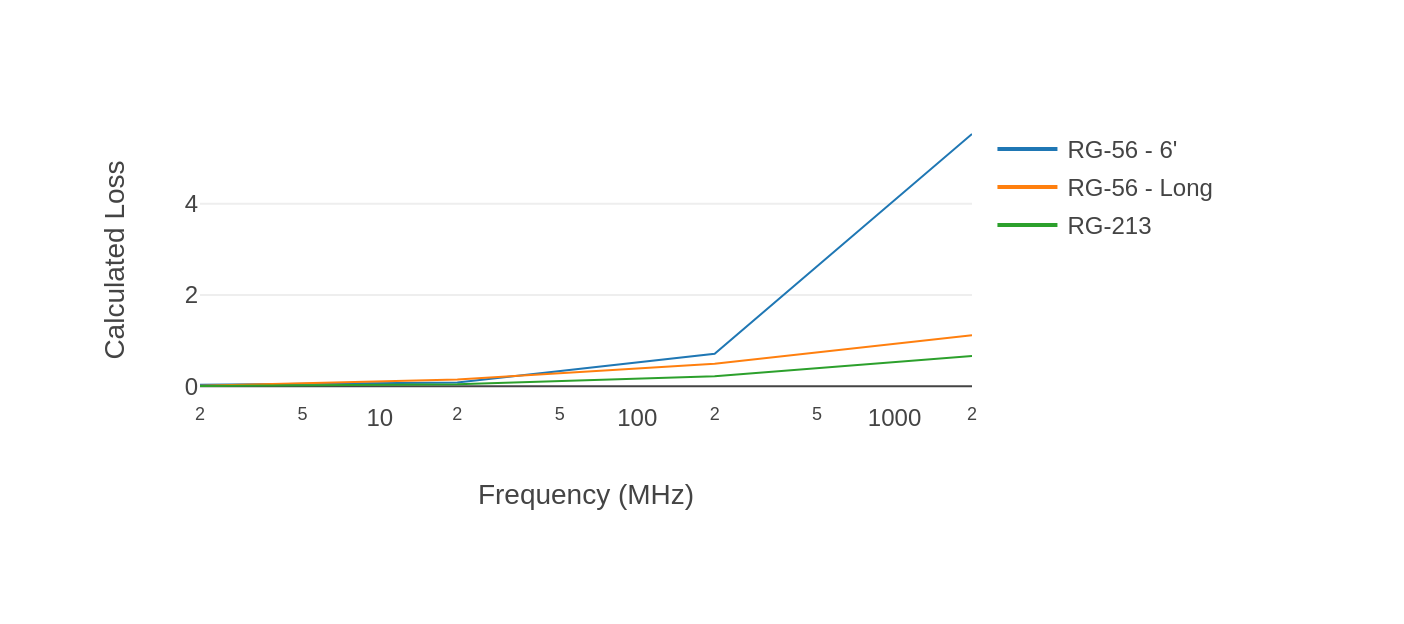
\includegraphics[width=0.6\textwidth]{CalculatedGraph.png}
\caption{Calculated Loss and Frequency}
\end{figure}
\newpage

\begin{center}
Lab Questions
\end{center}
\vspace{2mm}
\begin{enumerate}[label=\textbf{\arabic*.}]
\item To What degree are the losses affected by cable diameter and frequency? \\
Diameter and frequency have significant impacts on loss in transmission lines. As frequency increased, we noticed a marked increase in signal losses for both cable types. This is particularly noticeable in the RG-58 cable - its performance appeared to deteriorate rapidly as frequency increased. RG-213 on the other hand, demonsrtated much more consistant losses.
\item At what frequency does the cable type become critical? \\
We noticed losses start to escalate noticeably around 200 MHz for the RG-58, while RG-213 seemed to remain more consistant across the 2000 MHz range. This indicates that, starting at 200 MHz, it becomes more important which cable you choose.
\item Maximum Distance for each cable with a 100-Watt Transmitter and a 2-Watt Antenna \\
Max Loss(dB) = $10log(\frac{P_{in}}{P_{Out}} = 10log(50) = 16.99 dB$\\
Max Distance for RG-213 = $\frac{Max Loss}{a} = \frac{16.99}{0.22} = 77.2$ Meters \\
Max Distance for RG-68 = $\frac{16.99}{1.5} = 11.33$ Meters\\
\item Why are there multiple peaks? \\
This can be attributed to signal reflection within the transmission line.
When there is a fault or discontinuity in the line and a signal travelling down the line encounters this fault, a portion of the signal is reflected back and can interfere with the original signal, creating standing waves. It is these standing waves that result in peaks. 
\end{enumerate}

\end{document}
\end{document}